% Generated by scripts/report-data.mjs. Do not edit.
\definecolor{pc-P1}{HTML}{F17E7E}
\definecolor{pc-P2}{HTML}{7EF1A1}
\definecolor{pc-P3}{HTML}{C17EF1}
\definecolor{pc-P4}{HTML}{F1E37E}
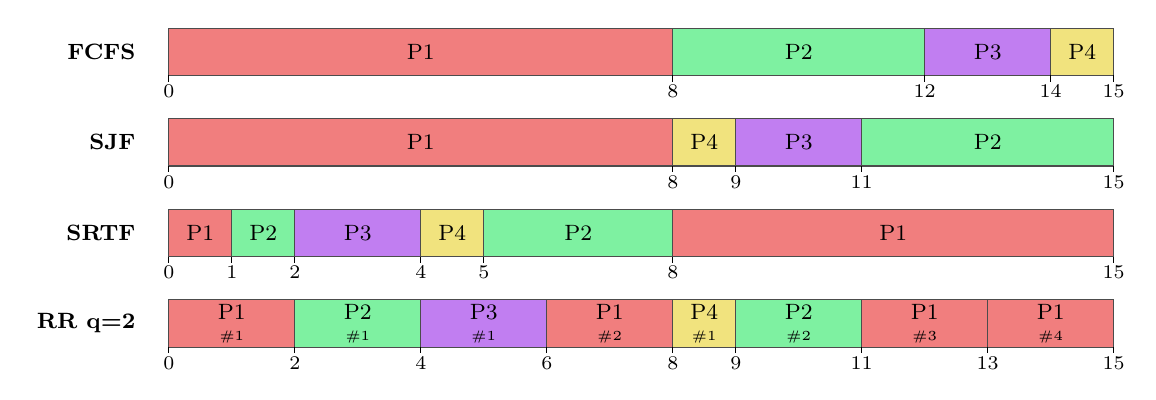
\begin{tikzpicture}[x=0.800cm, y=1cm, font=\footnotesize]
\node[anchor=east, font=\footnotesize\bfseries] at (-0.3/0.800, 0.3) {FCFS};
\draw[fill=pc-P1, draw=black!70] (0, 0) rectangle (8, 0.6);
\node[align=center, inner sep=0pt] at (4, 0.3) {P1};
\draw[fill=pc-P2, draw=black!70] (8, 0) rectangle (12, 0.6);
\node[align=center, inner sep=0pt] at (10, 0.3) {P2};
\draw[fill=pc-P3, draw=black!70] (12, 0) rectangle (14, 0.6);
\node[align=center, inner sep=0pt] at (13, 0.3) {P3};
\draw[fill=pc-P4, draw=black!70] (14, 0) rectangle (15, 0.6);
\node[align=center, inner sep=0pt] at (14.5, 0.3) {P4};
\draw (0, 0) -- (0, -0.08) node[below, inner sep=1pt, font=\scriptsize] {0};
\draw (8, 0) -- (8, -0.08) node[below, inner sep=1pt, font=\scriptsize] {8};
\draw (12, 0) -- (12, -0.08) node[below, inner sep=1pt, font=\scriptsize] {12};
\draw (14, 0) -- (14, -0.08) node[below, inner sep=1pt, font=\scriptsize] {14};
\draw (15, 0) -- (15, -0.08) node[below, inner sep=1pt, font=\scriptsize] {15};
\node[anchor=east, font=\footnotesize\bfseries] at (-0.3/0.800, -0.85) {SJF};
\draw[fill=pc-P1, draw=black!70] (0, -1.15) rectangle (8, -0.55);
\node[align=center, inner sep=0pt] at (4, -0.85) {P1};
\draw[fill=pc-P4, draw=black!70] (8, -1.15) rectangle (9, -0.55);
\node[align=center, inner sep=0pt] at (8.5, -0.85) {P4};
\draw[fill=pc-P3, draw=black!70] (9, -1.15) rectangle (11, -0.55);
\node[align=center, inner sep=0pt] at (10, -0.85) {P3};
\draw[fill=pc-P2, draw=black!70] (11, -1.15) rectangle (15, -0.55);
\node[align=center, inner sep=0pt] at (13, -0.85) {P2};
\draw (0, -1.15) -- (0, -1.23) node[below, inner sep=1pt, font=\scriptsize] {0};
\draw (8, -1.15) -- (8, -1.23) node[below, inner sep=1pt, font=\scriptsize] {8};
\draw (9, -1.15) -- (9, -1.23) node[below, inner sep=1pt, font=\scriptsize] {9};
\draw (11, -1.15) -- (11, -1.23) node[below, inner sep=1pt, font=\scriptsize] {11};
\draw (15, -1.15) -- (15, -1.23) node[below, inner sep=1pt, font=\scriptsize] {15};
\node[anchor=east, font=\footnotesize\bfseries] at (-0.3/0.800, -2) {SRTF};
\draw[fill=pc-P1, draw=black!70] (0, -2.3) rectangle (1, -1.7);
\node[align=center, inner sep=0pt] at (0.5, -2) {P1};
\draw[fill=pc-P2, draw=black!70] (1, -2.3) rectangle (2, -1.7);
\node[align=center, inner sep=0pt] at (1.5, -2) {P2};
\draw[fill=pc-P3, draw=black!70] (2, -2.3) rectangle (4, -1.7);
\node[align=center, inner sep=0pt] at (3, -2) {P3};
\draw[fill=pc-P4, draw=black!70] (4, -2.3) rectangle (5, -1.7);
\node[align=center, inner sep=0pt] at (4.5, -2) {P4};
\draw[fill=pc-P2, draw=black!70] (5, -2.3) rectangle (8, -1.7);
\node[align=center, inner sep=0pt] at (6.5, -2) {P2};
\draw[fill=pc-P1, draw=black!70] (8, -2.3) rectangle (15, -1.7);
\node[align=center, inner sep=0pt] at (11.5, -2) {P1};
\draw (0, -2.3) -- (0, -2.38) node[below, inner sep=1pt, font=\scriptsize] {0};
\draw (1, -2.3) -- (1, -2.38) node[below, inner sep=1pt, font=\scriptsize] {1};
\draw (2, -2.3) -- (2, -2.38) node[below, inner sep=1pt, font=\scriptsize] {2};
\draw (4, -2.3) -- (4, -2.38) node[below, inner sep=1pt, font=\scriptsize] {4};
\draw (5, -2.3) -- (5, -2.38) node[below, inner sep=1pt, font=\scriptsize] {5};
\draw (8, -2.3) -- (8, -2.38) node[below, inner sep=1pt, font=\scriptsize] {8};
\draw (15, -2.3) -- (15, -2.38) node[below, inner sep=1pt, font=\scriptsize] {15};
\node[anchor=east, font=\footnotesize\bfseries] at (-0.3/0.800, -3.15) {RR q=2};
\draw[fill=pc-P1, draw=black!70] (0, -3.45) rectangle (2, -2.85);
\node[align=center, inner sep=0pt] at (1, -3.15) {P1\\[-2pt]{\tiny\#1}};
\draw[fill=pc-P2, draw=black!70] (2, -3.45) rectangle (4, -2.85);
\node[align=center, inner sep=0pt] at (3, -3.15) {P2\\[-2pt]{\tiny\#1}};
\draw[fill=pc-P3, draw=black!70] (4, -3.45) rectangle (6, -2.85);
\node[align=center, inner sep=0pt] at (5, -3.15) {P3\\[-2pt]{\tiny\#1}};
\draw[fill=pc-P1, draw=black!70] (6, -3.45) rectangle (8, -2.85);
\node[align=center, inner sep=0pt] at (7, -3.15) {P1\\[-2pt]{\tiny\#2}};
\draw[fill=pc-P4, draw=black!70] (8, -3.45) rectangle (9, -2.85);
\node[align=center, inner sep=0pt] at (8.5, -3.15) {P4\\[-2pt]{\tiny\#1}};
\draw[fill=pc-P2, draw=black!70] (9, -3.45) rectangle (11, -2.85);
\node[align=center, inner sep=0pt] at (10, -3.15) {P2\\[-2pt]{\tiny\#2}};
\draw[fill=pc-P1, draw=black!70] (11, -3.45) rectangle (13, -2.85);
\node[align=center, inner sep=0pt] at (12, -3.15) {P1\\[-2pt]{\tiny\#3}};
\draw[fill=pc-P1, draw=black!70] (13, -3.45) rectangle (15, -2.85);
\node[align=center, inner sep=0pt] at (14, -3.15) {P1\\[-2pt]{\tiny\#4}};
\draw (0, -3.45) -- (0, -3.53) node[below, inner sep=1pt, font=\scriptsize] {0};
\draw (2, -3.45) -- (2, -3.53) node[below, inner sep=1pt, font=\scriptsize] {2};
\draw (4, -3.45) -- (4, -3.53) node[below, inner sep=1pt, font=\scriptsize] {4};
\draw (6, -3.45) -- (6, -3.53) node[below, inner sep=1pt, font=\scriptsize] {6};
\draw (8, -3.45) -- (8, -3.53) node[below, inner sep=1pt, font=\scriptsize] {8};
\draw (9, -3.45) -- (9, -3.53) node[below, inner sep=1pt, font=\scriptsize] {9};
\draw (11, -3.45) -- (11, -3.53) node[below, inner sep=1pt, font=\scriptsize] {11};
\draw (13, -3.45) -- (13, -3.53) node[below, inner sep=1pt, font=\scriptsize] {13};
\draw (15, -3.45) -- (15, -3.53) node[below, inner sep=1pt, font=\scriptsize] {15};
\end{tikzpicture}
